\chapter{Conclusions}\label{chap:conclusions}

After analyzing the data collected from the various experiments, I have clearly confirmed the election of a programming language does affect the performance and energy consumption. 

The program used to perform the benchmarks is an image renderer that processes each pixel of an image, casting multiple rays per pixel, and calculating the color of each one, using floating point operations, based on the intersection of the rays with the objects in the scene. This is a computationally intensive task that uses the \gls{ALU}, that can be parallelized.

This benchmark has been performed on the same component, the \gls{cpu}, even when performing the benchmarks on different platforms, such as a desktop computer, a laptop, and a \gls{SBC}.

I found that the most efficient programming language, by a great margin is \gls{CPP}, outperforming in every case. The results indicate that it outperforms both in energy consumption and execution time when compared to Go, a compiled language, and interpretations of languages, such as \gls{CPython} or PyPy. This was to be expected, as \gls{CPP} is a compiled language and is known for its performance and energy efficiency, being an evolution of C.


\section{Summary of Findings}
The main findings of this project are that \gls{CPP} is always faster and less consuming than any other language tested for a given platform and a specific core configuration, being up to $440$ times faster and $300$ times more energy efficient on the Server than \gls{CPython}, and up to $180$ times faster and $150$ times more energy efficient on the Raspberry Pi (the two extremes of the platforms used in this project).

An interesting result is that the lowest consuming board has been the Raspberry Pi, due to its design for IoT low-consumption devices. 

For each of the languages tested, the performance on up to 4 cores on each platform, limited to 60 seconds, is detailed on this graph:

%% Conclusion figure without python
\hypertarget{fig:conclusion-scatter-nopy}{} % anchor for links
% \begin{adjustbox}{max width=\textwidth}
    \begin{figure}[h]
        \centering
        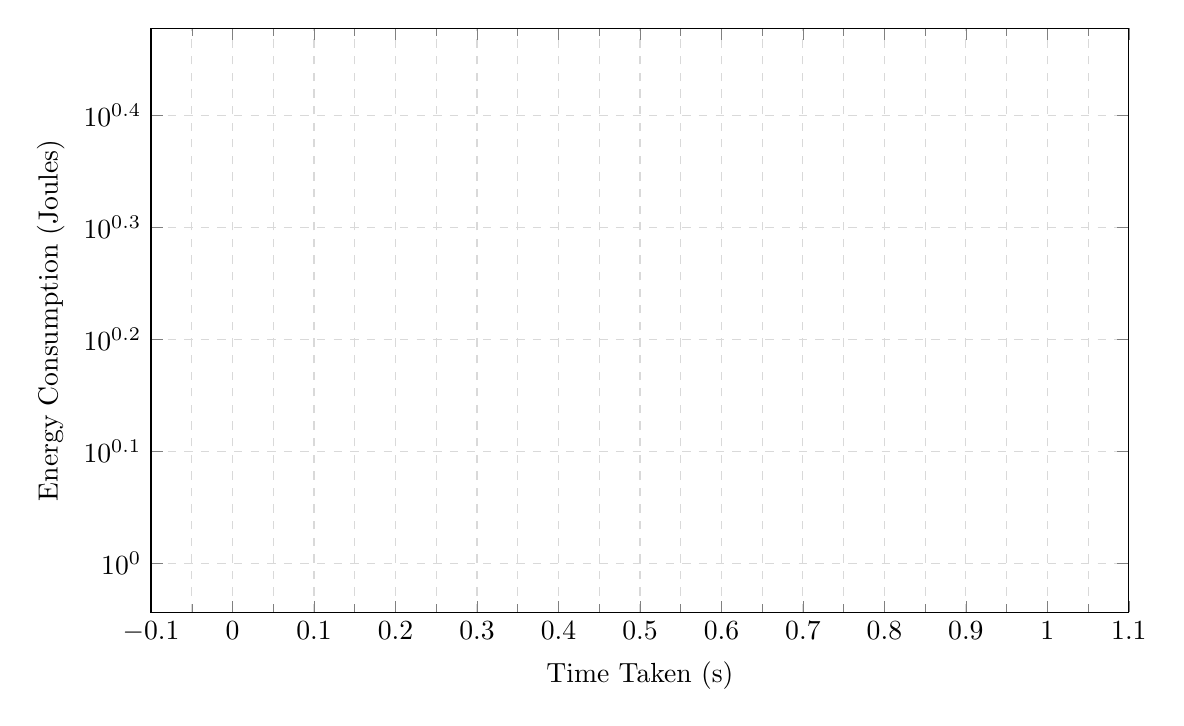
\begin{tikzpicture}
            \begin{axis}[
            width=14cm, height=9cm,
            xlabel={Time Taken (s)},
            ylabel={Energy Consumption (Joules)},
            ymode=log,
            xmin=0, xtick={0,20,40,60,80,100,120,140,160,180,200,220,240,260},
            % enlarge x limits=false,
            grid=both, minor tick num=1,
            grid style={gray!30,dashed},
            legend style={at={(0.5,1.05)},anchor=south,legend columns=-1, draw=none},
            enlargelimits=0.1,
            clip=false
            ]
            % plots (no Python)
            \PlotCXXconclusion
            \PlotGoconclusion
            \PlotPyPyconclusion
            \legend{C++, Go, PyPy}

            % clickable "button" back to the full plot
            \node[anchor=north east, fill=gray!15, draw, rounded corners,
                    inner sep=3pt] at (axis description cs:0.98,0.98)
                                {\hyperref[chap:appendix-scatter-plot]{\strut Show \emph{with} Python}};
            \end{axis}
        \end{tikzpicture}
    \caption[Scatter plot of C++, Go, and PyPy.]{The plot shows the relationship between time taken and energy consumption for each programming language. The data points represent different implementations, where the label has the form X-Y, with X being the platform and Y being the number of cores used.}
    \label{fig:conclusion-scatter-nopy}
    \end{figure}
% \end{adjustbox}

In all cases, we can observe that the python results lie at a large distance from the other programming languages, arround $100$ times lower, indicating a significant performance gap. This is due to the fact that \gls{CPython} is an interpreted language, without \gls{jit} compilation, and with a \gls{GIL} that limits the performance. For the other programming languages, the order in which they appear in the graphs is the same in all cases, being C++ the fastest, then PyPy and finally Go. Except for three specific cases: the Raspberry Pi energy consumption and execution time at 4 cores, where Go is faster than PyPy in both scenarios (\autoref{fig:rpi-relative-combined}) and on the energy consumption of the \gls{ram} on the server benchmark, using 28 or more cores, where Go is more efficient than PyPy (\autoref{fig:log-server-energy-ram}).

With respect to the wattage consumption, we can see that the laptop, although it has its power limited to less than 60W, the wattage consumption does not increase when allowing the program the use of all 14 cores compared to only 10, which might be due to the fact that the platform has 10 High-Performance cores and 4 Efficiency cores. It is also interesting, with respect to this platform, that the energy consumption is always the same, on every core configuration, for any given programming language.



\section{Discussion of Results}

% Move this to a different section
The most impressive and surprising result for many tests has been the performance of PyPy compared to the other programming languages. PyPy is just an interpreter for Python (that can run a limited subset of what \gls{CPython} can run), but it uses a \gls{jit} compilation technique that allows it to execute Python code much faster than the standard interpreter. This \gls{jit} is not compatible with some Python libraries such as Numpy \cite{numpy} as these libraries use \gls{c-extension} to speed up \gls{CPython}'s speed. This means that PyPy can only be used with pure Python code, which limits its applicability in some cases.

The implementation of multiple threads in the different programming languages was also a key factor in the performance of the programs. Depending on the technique used, parallelizing for each line or for each pixel, the performance deferred on the different languages. The easiest to implement, and the one that showed the best results, was C++, followed by Go, with its \glspl{goroutine} and \glspl{channel}. Python's default implementation, \gls{CPython}, does not support true multithreading due to the \gls{GIL}, which limits the performance of multi-threaded programs, thus, the need of the library multithreading is needed.


It can be observed that as the program has access to more cores, both the the energy consumption and the execution time decrease. We can also see that when comparing multithreaded performace compared to single-threaded performance, the results tend to stabilize after 8/16 cores, depending on the platform, which follows Amdahl's law (\cite{amdahl:law}), which states that: 
$$
S = \frac{1}{(1 - P) + \frac{P}{N}}
$$
Where $S$ is the speedup, $P$ is the parallelizable portion of the program, and $N$ is the number of cores. This is due to the fact that the program has a portion that is not parallelizable (the creation of the world and instantiation of the speheres), and as the number of cores increases, the impact of this portion becomes more significant.

If I were to use libraries such as \Gls{numpy}, the performance of \gls{CPython} would be much better, as these libraries are optimized for performance and can take advantage of the underlying hardware. However, this would not be a fair comparison, as we would not be using pure Python code.

If I was to deploy a render-farm, with this program, I could be paying 300x less energy costs if I used \gls{CPP} instead of \gls{CPython} or Go, and renders could take up to 400x less time. This is a significant difference, and it is clear that \gls{CPP} is the best choice for these types of application.

There is an interesting outlier in this analysis, which are the results of PyPy on the laptop. Specifically, if we look at the results of the relative energy efficiency (\autoref{fig:laptop-relative-energy}), we can see that PyPy, as the number of cores increase, the relative energy efficiency decreases, while the other programming languages increase. This seems to indicate that PyPy is not able to take advantage of the multiple cores in the laptop as well as other platforms. I have some possible ideas on why this might happen; My first hypothesis was that the implementation being used on the laptop was an emulation of the x86 version of PyPy using Rosetta 2 (\cite{apple:rosetta2}), but when checking the `Activity Monitor', it is clear that this process is native to \gls{ARM}.\@ My second hypothesis is that this is due to the fact that, as this is one of the platforms that does not use x86 architecture, the \gls{jit} compilation is not as effective.


In conclusion, if the program is to be run only a couple of times, and the performance is not a key factor, \gls{CPython} is a good enough choice because of its ease of use and development speed. However, if the program is to be run multiple times, or if performance is a key factor, \gls{CPP} is the best choice. Go is also a good choice, as it has a good balance between performance and ease of use, specially for hundreds of threads working light tasks, for example a web server. PyPy is a good choice for pure Python code, but it has limitations when it comes to libraries that use \glspl{c-extension}.

This comes as an interesting conclusion, as when I think about a program or funciton that has to be run multiple times, I think about a web serverless function, for example AWS Lambda (\cite{aws:lambda}), but in the \href{https://docs.aws.amazon.com/lambda/latest/dg/lambda-samples.html}{examples} they provide, there is no mention either of PyPy or C++. The main focus they have is Node.js (a JavaScript runtime), Python, Ruby, Java, and, in fifth place, Go. This is an interesting choice, as it seems that the focus is on ease of use rather than performance. I think this is also due to the fact that these services charge by execution time, so the slower the execution time, the more they can charge the custumer. 


\section{Directions for Future Research}
Future research could focus on the following areas:
\begin{itemize}
    \item Investigating the performance of other programming languages, such as Rust, Javascript, or Java, in similar scenarios.
    \item Exploring the impact of different libraries and frameworks on the performance of the programming languages.
    \item Analyzing the performance external accelerators such as \gls{gpu} or \gls{fpga} in conjunction with the programming languages, such as Numpy
    \item Conducting a more extensive analysis of the performance of the programming languages in different scenarios, such as web applications, data processing, or machine learning.
    \item Analyzing more workloads, such a web-server or a database, to see how the programming languages perform in these scenarios.
    \item Investigating the impact of different hardware configurations on the performance of the programming languages such as the \gls{ram} speed, size and SSD storage speed.
    \item Exploring the impact of different operating systems on the performance of the programming languages, such as Linux, Windows or macOS on the same hardware.
\end{itemize}